%%%%%%%%%%%%%%%%%%%%%%%%%%%%%%%%%%%%%
%% Supporting Information
%% (Optional)
%%%%%%%%%%%%%%%%%%%%%%%%%%%%%%%%%%%%%
% OVERVIEW
%
% Please note that all supporting information will be peer reviewed with your manuscript.
% In general, the purpose of the supporting information is to enable
% authors to provide and archive auxiliary information such as data
% tables, method information, figures, video, or computer software,
% in digital formats so that other scientists can use it.

% The key criteria are that the data:
% 1. supplement the main scientific conclusions of the paper but are not essential to the conclusions (with the exception of
%    including data so the experiment can be reproducible);
% 2. are likely to be usable or used by other scientists working in the field;
% 3. are described with sufficient precision that other scientists can understand them, and
% 4. are not exe files.
%

% All Supporting text and figures should be included in this document.

% Data sets, large tables, movie files,
% and audio files should be uploaded separately, following AGU naming
% conventions. Include their captions in this document and list the
% file name with the caption. You will be prompted to upload these
% files on the Upload Files tab during the submission process, using
% file type “Supporting Information (SI)”

%\documentclass{agujournal2018}

\documentclass[main.tex]{subfiles}


% Please type in the journal name: \journalname{<Journal Name>}
% ie,
%\journalname{Geophysical Research Letters}

%% Choose from this list of Journals:
%
% Journal of Geophysical Research
% JGR-Biogeosciences
% JGR-Earth Surface
% JGR-Planets
% JGR-Solid Earth
% JGR-Space Physics
% Global Biochemical Cycles
% Geophysical Research Letters
% Paleoceanography
% Radio Science
% Reviews of Geophysics
% Tectonics
% Space Weather
% Water Resource Research
% Geochemistry, Geophysics, Geosystems
% Journal of Advances in Modeling Earth Systems (JAMES)
% Earth's Future
% Earth and Space Science

\begin{document}

%% This command needs article title as argument to \supportinginfo{}:
%\supportinginfo{A Low Cost Fiber-Optic Displacement Sensor Designed For Use at High Pressure}

%\authors{Eric Burdette and Greg Hirth}


%\affiliation{1}{Department of Earth, Environmental and Planetary Sciences, Brown University, Providence, RI, USA}

%% Corresponding Author
%(include name and email addresses of the corresponding author.  More
%than one corresponding author is allowed in this Word file and for
%publication; but only one corresponding author is allowed in our
%editorial system.)  

%\correspondingauthor{Eric Burdette}{eric\_burdette@brown.edu}

%% ------------------------------------------------------------------------ %%
%
%  TEXT
%
%% ------------------------------------------------------------------------ %%

% \section*{Contents}
% %%%Remove or add items as needed%%%
% \begin{enumerate}
% \item Text S1 to Sx
% \item Figures S1 to Sx
% \item Tables S1 to Sx
% \end{enumerate}

% \section*{Additional Supporting Information (Files uploaded separately)}

% \begin{enumerate}
% \item placeholder
% \end{enumerate}

% \section*{Introduction}
%     Here we have included supporting details describing details of other configurations in which the sensor can be used, and practical modifications made to the pressure vessel and support baseplate to incorporate the EFPI into our apparatus.
%Delete all unused file types below. 
%Copy/paste for multiples of each file type as needed.

\section{Supporting Information}

\subsection{Temperature Sweep Displacement Tracking}
        With the same components, a laser die temperature sweep can change wavelength by more than a nanometer to cross several fringes of the Fabry-Perot cavity. The approach is slow, requiring 8 seconds for a single wavelength scan cycle, but it allows calculation of the absolute cavity length. Figure \ref{fig:CH4s_TempScan} shows scans at 10 MPa and 50 MPa. Fringe spacing changes slightly, by a factor of $\Delta\sigma/E$. The position of the fringes, or alternatively the wavelength spectra of the cavity, is recorded over time and displayed in Figure \ref{fig:CH4s_TemperatureScans_wloading}, along with the modelplots of equation \ref{eq:CH4_e1} considering displacement on the loaded 10 mm alumina elastic element and temperature dependent wavelength.
\begin{figure}
  \includegraphics[width=\textwidth]{Figures/Scan_success1_10vs50_Wavescan.pdf}
  \caption{Data from an unconfined elastic loading experiment. Scans were taken at 10 MPa and 50 MPa axial loads. 
  }
  \label{fig:CH4s_TempScan}
\end{figure}

\begin{figure}
  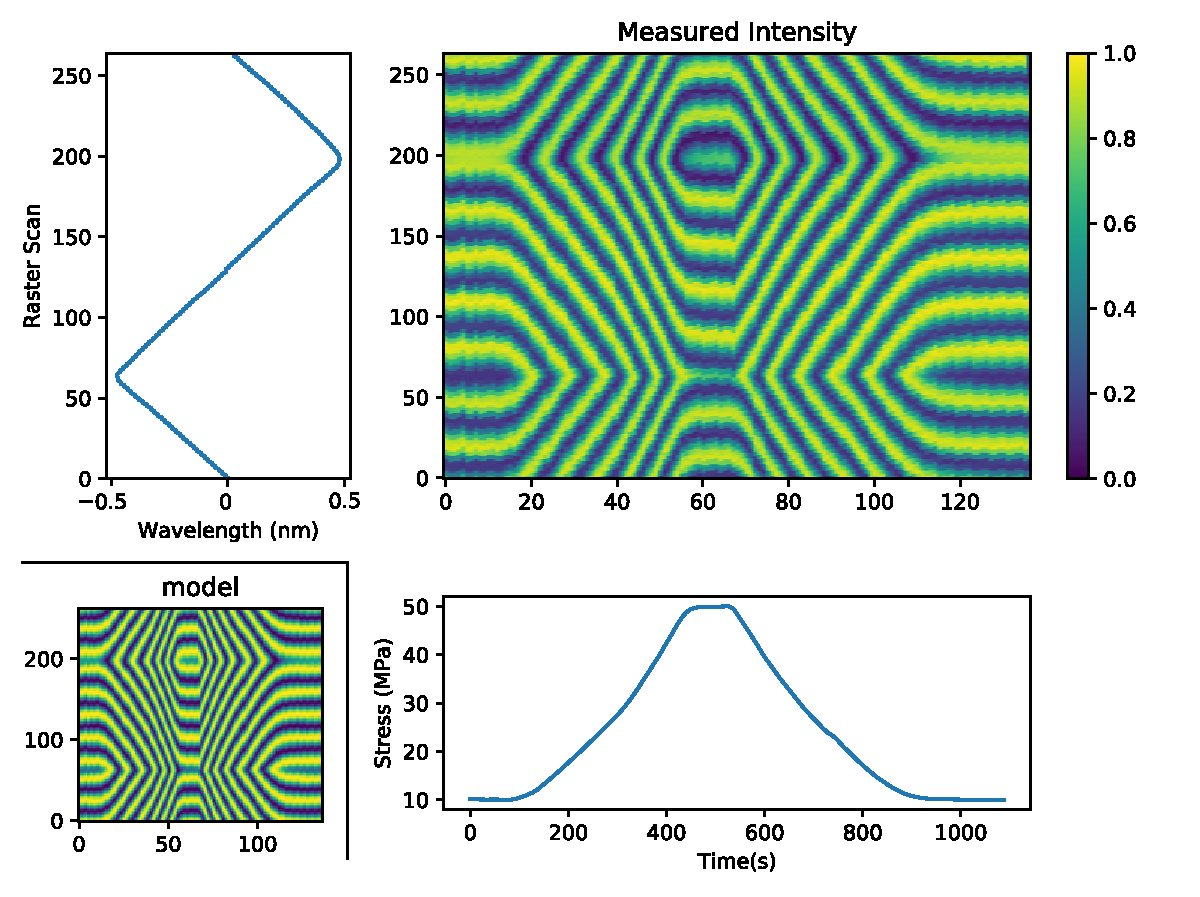
\includegraphics[width=\textwidth]{Figures/Scan_success1_wmodel2.pdf}
  \caption{Plots of temperature scans recorded during a ramp in load. Fringes pass in the horizontal (x, time) direction for a given wavelength (y) as they would for the direct (frequency f) amplitude in the current modulated design. 
  }
  \label{fig:CH4s_TemperatureScans_wloading}
\end{figure}    



\subsection{Vibrometer Modifications}
    A vibrometer can easily be incorporated into the design of the interferometer if optocouplers and another leg (e.g. fiber) are added to mix returning light with the incident, modulated signal. The sensor face needs and anti-reflective coating to avoid Fabry-Perot effects. I-Q demodulation can be used to track the position of the reflector to higher speeds.


\subsection{Use at High Temperature}
    \begin{figure}
      \includegraphics[width=\textwidth]{Figures/Thermal_model_baseplate_Compare-ThesisEdits_small.pdf}
      \caption{Thermal model comparing an assembly with ceramic outer pieces to a modified assembly with material changes. Temperatures at the surface of the baseplate drop by 80°C, allowing a feasible implementation of a glued Fabry-Perot cavity.}
      \label{fig:CH4s_ThermalModel1}
    \end{figure}
    \begin{figure}
      \includegraphics[width=\textwidth]{Figures/New_Baseplate_section.PNG}
      \caption{Cross section of re-designed baseplate.}
      \label{fig:CH4s_NewBaseplate_Section}
    \end{figure}
    \begin{figure}
        \includegraphics{Figures/New_Baseplate_Orthogonal.PNG}
        \caption{Orthogonal view of re-designed baseplate.}
        \label{fig:CH4s_NewBaseplate_Section_orth}
    \end{figure}
    High temperature deformation in a Griggs-type apparatus is a challenging environment, with sample temperatures up to 1200°C less than 2 cm from the exterior of the pressure vessel. Existing pressure vessel and assembly design choices are mostly a legacy from eras when numerical modeling was inaccessible, which has made some thermal problems intractable to solve.
    To insert the ferrule ~1 cm from the hot sample requires adequate water cooling close to the sample to keep temperatures below fiber epoxy temperature limits of 100°C. Adding cooling tubes/channels sacrifices metal required to support the sample and pressure vessel. To explore the design space we developed a 2D axisymmetric thermal model published in Moarefvand et al (2021), and modified it to include a 'baseplate' supporting the pressure vessel, with heat transfer coefficient boundary conditions to water representing our actual cooling conditions rather than the simplified fixed temperature commonly used.
    We find that:
    \begin{enumerate}
        \item Assembly material thermal conductivity (inside the pressure vessel) has a large effect on required power, and governs pressure vessel inner wall temperature. Changing from sodium chloride to potassium bromide confining media would decrease thermal conductivity by a factor of two and reduce vessel temperatures from 180°C to 100°C at 700°C sample temperatures.
        \item Current water cooling is inadequate below the pressure vessel. While water channels on top of the pressure vessel have a 1" ID and 3" OD with a 1/4" height, cooling in the baseplate is provided by a single 1/8"ID, 1/4" OD copper tube. This leads to high temperatures extending below the sample, with the baseplate reaching ~160°C at 700°C sample temperatures.
        \item Current materials conduct along the central axis (tungsten carbide), and insulate near the pressure vessel walls (pyrophyllite) where the water cooling is placed (see model). This leads to heat flowing downward into the baseplate, and then outward towards water cooling which further increases temperatures in the base carbide where the ferrule is placed. This can be swapped, putting steel near the vessel, and using a central pillar of zirconia or alumina (Figure \ref{fig:CH4s_ThermalModel1}. Several european groups modified their assemblies to this design \citep{rybacki1998servohydraulically} but do not note this benefit.
    \end{enumerate}
    
    In addition to the planned changes to the salt used for confining media and changes to the lower insulating material, we redesigned a baseplate to incorporate large water channels and a high conductivity beryllium copper support core (Figure \ref{fig:CH4s_NewBaseplate_Section}, \ref{fig:CH4s_NewBaseplate_Section_orth}). We took the opportunity to add an axisymmetric cavity at the bottom of the support post to incorporate acoustic emission sensors.
    


\end{document}